
% Puts a line after the Chapter Heading
\vspace{-1cm}\noindent\rule{\textwidth}{0.4pt}

\section{Background of the Study}
% Introductory Paragraph
% Background to Agriculture

Agriculture plays a major role in feeding billions of people all
across the globe. It has also provided a means for people
to grow revenue and sustain their lives. In fact according to the 
World Bank Organization, "Agricultural development 
is one of the most powerful tools to end extreme poverty, 
boost shared prosperity and feed a projected 9.7 billion people by 2050.
Agriculture plays an integral 
part of the Philippine Economy, 
in fact according to the Philippine Statistics Authority, the Gross 
Value Added (GVA) in agriculture of the year 2019
is valued at 1.78 Trillion Pesos. 
It also contributes to the diet of Filipinos producing various 
ingredients of that are necessary for the Filipino Cuisine such as rice 
being the staple ingredient and other leafy vegetables such as cabbage,
saluyot and ampalaya. \\


% Further discussions introducing the Problem/Issues
% Intoduce problems 

Each year, farmers spend a lot of money on disease management, they 
often do so without proper technical support leading poor disease 
control, pollution and harmful result. Plant diseases cause 
substantial loss to farmers resulting to large economic loss.
That's why accurate identification and diagnosis of plant diseases is 
essential; especially now in the era of globalization and climate 
change. \\

During the past few years, there has been a rapid advancement to the
area of Machine Learning. Because of this there are now self-driving cars 
that can fully control a vehicle with minimal efforts required from the
driver. Engineers and researchers have achieved this through the use 
of different types of Neural Networks. \\

Convolutional Neural Network is a type of Neural Network that specializes 
in finding patterns to images. It is being used in almost all areas of science, 
for instance (Hadush et al.) has used CNNs to detect breast 
cancer from mammogram(MG) images achieving a detection accuracy 91.86\%. 
(Elgammal et al.) used CNNs to perform weather classification achieving 
82.2\% normalized classification accuracy.
\\

% Breast Cancer -> https://arxiv.org/abs/2003.07911
% Weather Classification -> https://www.researchgate.net/figure/Weather-Prediction-CNN-Architecture-Our-Neural-network-follow-the-CNN-layer_fig1_280218749

This study aims to develop a mobile application that uses a 
CNN Model  to detect and classify potential diseases in 
plants. Due to the current pandemic, the researcher decided to use publicly 
available image datasets — which will be used to train several CNN Models 
that would be embedded in the application — instead of making one. The researcher 
found publicly available image datasets of the following plants:
apple, cherry, citrus, corn, grape, peach, pepper, potato,
rice, strawberry (this selection is tentative). These images of different types 
of plants will be used to train the CNN Model and be able to detect diseases from 
these plants using an image of the plant leaves. \\ 

Because the model inference will
happen on the device itself without relying on a cloud-based server, 
farmers and other people would be able to input an image to this application 
and use this app and diagnose a plant without having to rely on an 
existing data or internet connection. This is important since according to 
the  National ICT Household Survey,which was conducted by the Philippine Statistical 
Research and Training Institute and the Philippine Statistics Authority, only 
17.7 \% of all households in the Philippines have Internet connection. 

% Internet Study -> https://businessmirror.com.ph/2020/12/01/itu-flags-connectivity-gaps-internet-access-in-philippines-other-nations/

\newpage 


\section{Theoretical Framework}
% TODO 
% 1. Bolster the statements using studies 

\begin{figure}[h!]
      \centering
      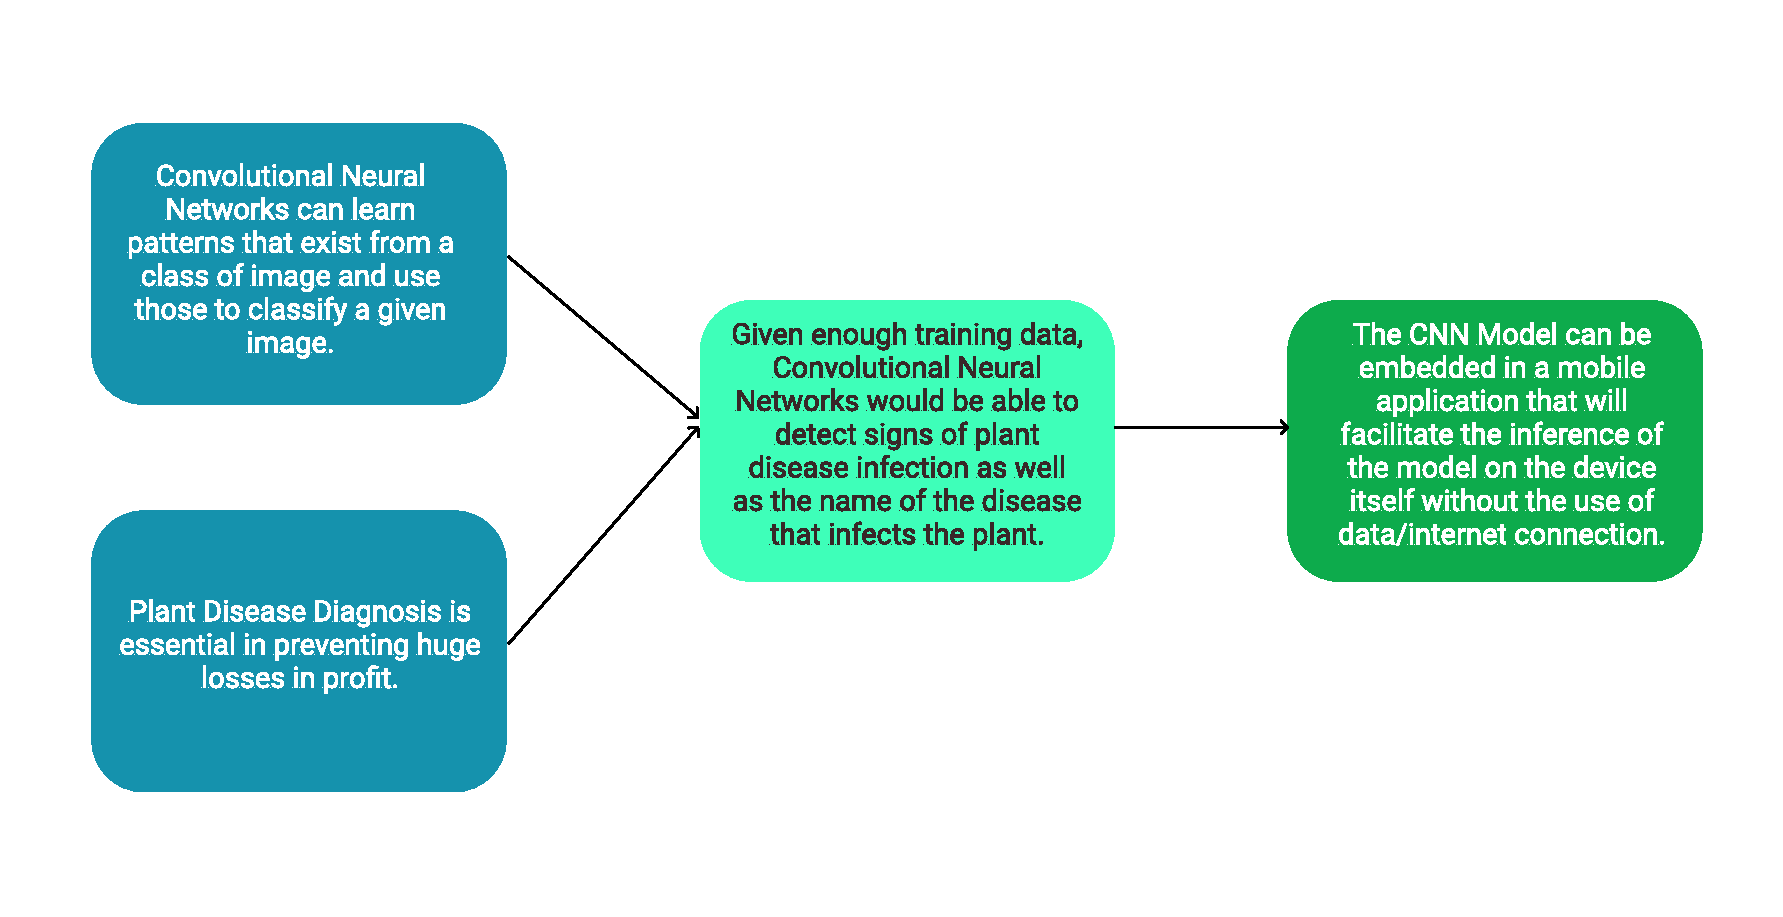
\includegraphics[scale=0.5]{01-intro-theoretical-framework.pdf}
      \caption{The Theoretical Framework of the Study}
\end{figure}

Convolutional Neural Networks has been experimentally shown 
to detect certain patterns from images with a high degree of 
accuracy. This is accomplished 
by feeding the CNN Model with labeled images and allowing it to "learn"
the existing patterns from these images which will grant in the ability 
to infer the classification a given image later on. This concept 
can be applied to plant diagnosis by training a CNN Model using a database 
of different types of healthy and infected plants. Since the CNN Model 
will be able to learn these patterns and detect if it the input image is 
healthy or infected as well as the name of the disease infecting the plant. \\


Plant disease diagnosis is essential in agriculture. Without proper 
identification of the disease and the disease-causing agent, disease 
control measures like pesticides can lead to further losses in time,
money and may even lead to more plant losses. This is why it is essential
to diagnose plants early on. \\ 

\section{Conceptual Framework}

\begin{figure}[H]
      \centering
      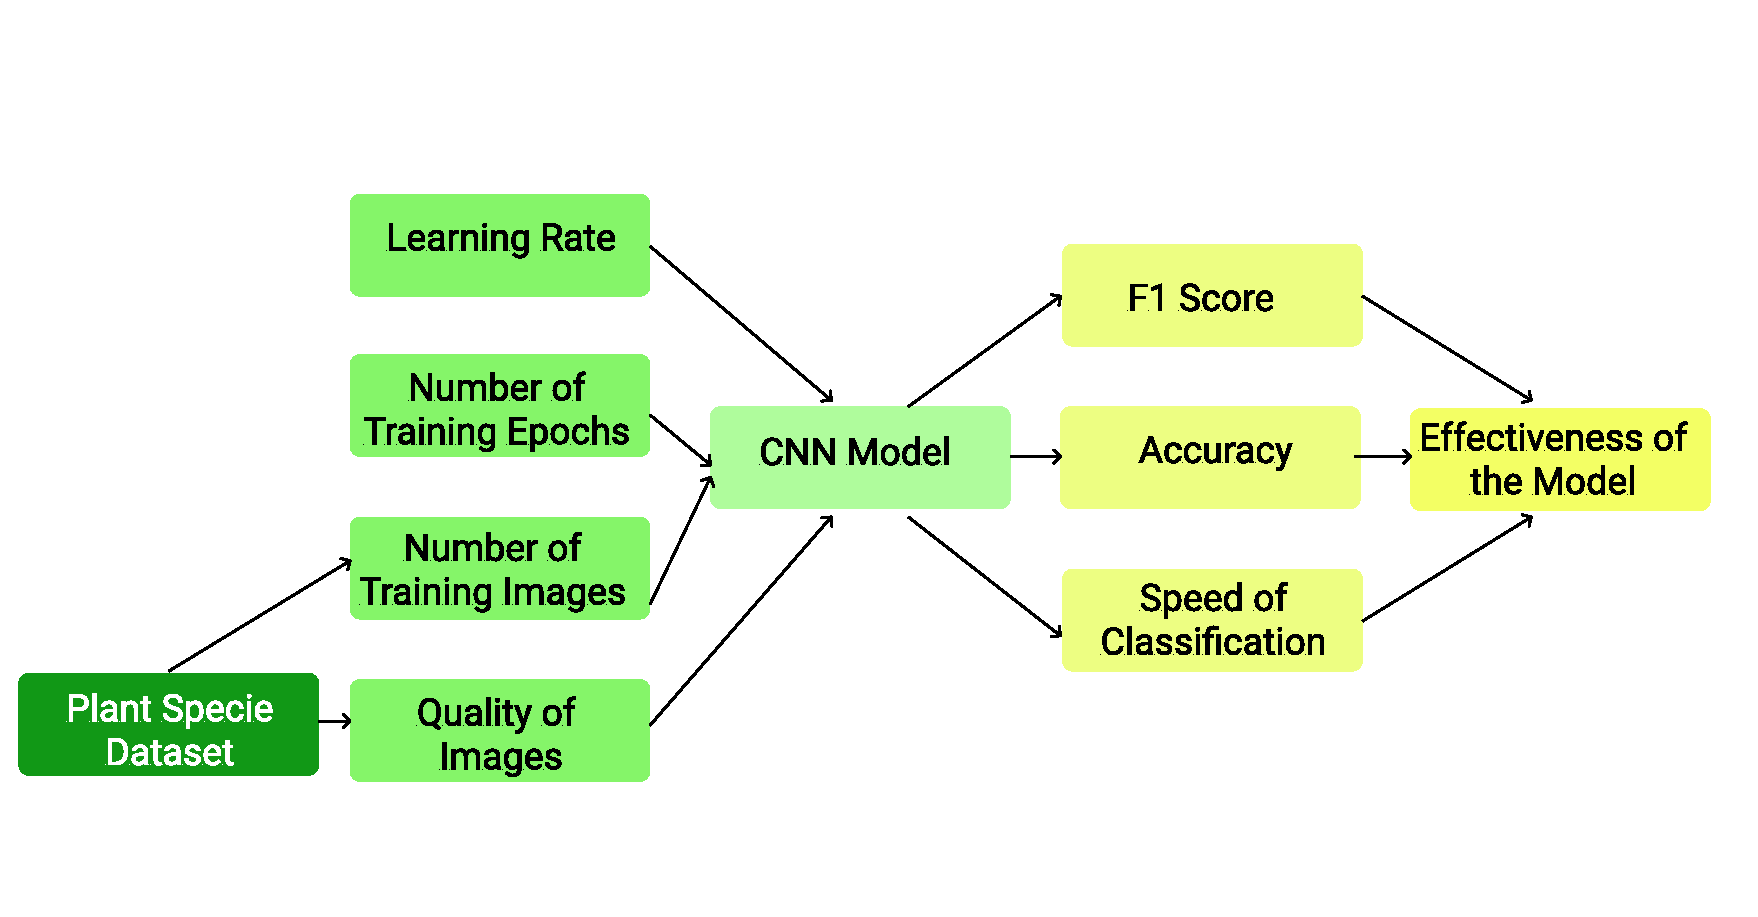
\includegraphics[scale=0.5]{01-intro-conceptual-framework.pdf}
      \caption{The Conceptual Framework of the Study}
\end{figure}

This study focuses on achieving the optimal effectiveness of the CNN Model that 
will be embedded in the mobile application. \\ 

In evaluating the effectiveness of a Neural Network Model 
one metric that is used is the F1 Score. It is defined as the harmonic mean 
of Precision and Recall or phrased mathematically as:
\[ 
 \text{F1 Score} \: = \: \frac{2}{\frac{1}{\text{Precision}} \: + \: 
\frac{1}{\text{Recall}}} 
\]

In addition to the F1 Score, accuracy will also be used as a metric to 
quantify the effectiveness of the model. It is defined as:
\[
      \text{Accuracy} \: = \: \frac{\text{Precision} \: + \: 
      \text{Recall}}{\text{Total Number of Test Images}}
\]

Finally, the speed of classification will also be used to 
gauge the effectivenes of the model. These 3 metrics will be used 
quantitatively measure the effectivenes of the model. \\

During the training process of the Model, there will be intervening variables 
that this study will not consider these are: Number of Training Epochs, 
Number of Training Images, Learning Rate, Quality of Training Images.




\section{Statement of the Problem}

    \begin{enumerate}
    \item How effective is the model in predicting the
    type of disease present in the given image? 
    In terms of:

        \begin{enumerate}
            \item Accuracy
            \item F1 Score 
            \item Speed of Classification 
        \end{enumerate}

    \item How comparable is the model made by the researcher 
    to other methods of detecting plant disease? 
    \end{enumerate}

\section{Hypotheses}
    \begin{enumerate}
        \item The F1 Score and the Speed of Classification implies that
              the model is not effective in predicting the tyoe of disease 
              present in the given image.
        \item The model is not comparable to other methods of detecting plant
              disease.
    \end{enumerate}

\section{Scope and Delimitation}
This study will only focus to the effectiveness of 
CNN Models to diagnose the following plants 
apple, cherry, citrus, corn, grape, peach, pepper,
potato, rice, strawberry (this selection is tentative). 
This is due to the fact that without training data on a 
certain type of plant CNN Models will be inconclusive with 
regards to the diagnosis of that specific plant. \\

This study does not include the effects of these factors: Number of Training Epochs, 
Number of Training Images, Learning Rate, Quality of Training Images 
that may affect the training and effectivess of the model. 

\section{Significance of the Study}
The significance of the study lies on the
fact that plant disease diagnosis plays a huge role 
in minimizing the monetary and material loss in
agriculture caused by various plant diseases.  
That’s why proper plant disease diagnosis is a
detrimental process in securing the value of 
crops grown. The study proposes an application 
that can be used to scan images of plant leaves 
which would then be used to detect various plant 
diseases which may be present in an image, this 
application is designed to run the disease diagnosis 
without the need of internet or data connection.
This study would certainly benefit farmers who 
have no access to internet connection to diagnose
their plants and prevent further crop losses. 


\section{Definition of Terms}
    \begin{itemize}
        \item Model \\
              - A machine learning model is a file that has
              been trained to recognize certain types of patterns.
              You train a model over a set of data, providing it an
              algorithm that it can use to reason over and learn 
              from those data.

        \item Convolutional Neural Networks \\
              - A Convolutional neural network (CNN) is a neural network 
              that has one or more convolutional layers and are used mainly
              for image processing, classification, segmentation and also 
              for other auto correlated data.

        \item Gross Value Added \\
              - Gross value added is the measure of the value of 
              goods and services produced in an area, industry or sector 
              of an economy.

        \item F1 Score \\
              - The F-score, also called the F1-score, is a measure of a model's accuracy 
              on a dataset. A good F1 score means that you have low false positives and 
              low false negatives, so you're correctly identifying real threats and you are not disturbed by false alarms
              
        \item Machine Learning \\
              - Machine learning is an application of artificial intelligence 
              (AI) that provides systems the ability to automatically learn and
              improve from experience without being explicitly programmed. 
              Machine learning focuses on the development of computer programs 
              that can access data and use it to learn for themselves.

        \item Classification \\
              - Classification refers to a predictive modeling problem where a
              class label is predicted for a given example of input data.
              
        \item Inference \\
              -  Inference refers to the process of using a trained machine learning algorithm to make a prediction

        \item Recall \\
              - Recall (also known as sensitivity) is the fraction of relevant instances that were retrieved.

        \item Precision
              - precision (also called positive predictive value) is the fraction of relevant instances among 
              the retrieved instances.
      
        \item Learning Rate \\
              - Learning rate is a tuning parameter in an optimization algorithm that determines the step size
               at each iteration while moving toward a minimum of a loss function.     
            
        \item Epoch \\
              - epoch is a term used in machine learning and indicates the number of passes of the entire
               training dataset the machine learning algorithm has completed. 
    \end{itemize}


